\begin{frame}
  \frametitle{1D Chain of Atoms --- 2 Atoms per Unit}
  A 1D chain with 2 atoms in each unit: $R_{j}^s(t) = x_j + d_s + u_{j}^s(t);\quad s=1,2$
  \begin{center}
    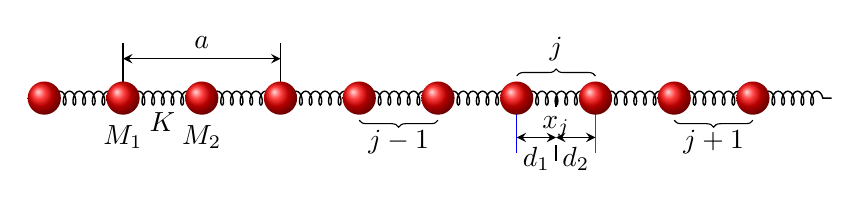
\begin{tikzpicture}
      [
      spring/.style={
        line width=0.5pt,
        decorate,
        decoration={
            coil,
            amplitude=2.5,
            segment length=3.5,
          }
        },
      ]
      \draw[line width=0.5pt] (1.0, 0.0) -- (1.0, 0.7);
      \draw[line width=0.5pt] (3.0, 0.0) -- (3.0, 0.7);
      \draw[line width=0.5pt, <->, >=stealth] (1.0, 0.5) -- node[pos=0.5, anchor=south] {$a$} (3.0, 0.5);

      \draw[line width=0.5pt, draw=black] (6.5, 0.0) -- (6.5,-0.8);
      \draw[line width=0.5pt, draw=blue] (6.0, 0.0) -- (6.0,-0.7);
      \draw[line width=0.5pt, draw=red] (7.0, 0.0) -- (7.0,-0.7);

      \node[below=3pt, fill=white] at (6.5, 0.0) {$x_j$};
      \draw[line width=0.5pt, <->, >=stealth] (6.0,-0.5) -- node[pos=0.5, anchor=north] {$d_1$} (6.5,-0.5);
      \draw[line width=0.5pt, <->, >=stealth] (6.5,-0.5) -- node[pos=0.5, anchor=north] {$d_2$} (7.0,-0.5);

      \node[anchor=center] at (1, -0.5) {$M_1$};
      \node[anchor=center] at (2, -0.5) {$M_2$};
      \node[] at (1.5,  -0.3) {$K$};

      \draw[decorate, decoration={brace, mirror, raise=8pt}] (4.0, 0.0) --
      node[pos=0.5, below=8pt] {$j-1$}(5.0, 0.0);
      \draw[decorate, decoration={brace, raise=8pt}] (6.0, 0.0) --
      node[pos=0.5, above=10pt] {$j$}(7.0, 0.0);
      \draw[decorate, decoration={brace, mirror, raise=8pt}] (8.0, 0.0) -- 
      node[pos=0.5, below=8pt] {$j+1$}(9.0, 0.0);

      \foreach \x in {0,1,...,9}{
        % draw the spring
        \draw[spring, draw=black] (\x, 0) -- ++(1, 0);
        % draw the atoms
        \ifthenelse{\x > 0}
        {
          \pgfmathparse{int(mod(\x, 2))}
          \let \n = \pgfmathresult
          \ifthenelse{\n = 0}{
            \shade[ball color=blue] (\x, 0) circle (5pt);
          }{
            \shade[ball color=red] (\x, 0) circle (6pt);
          }
        }{}
      }
    \end{tikzpicture}
  \end{center}
  The Newton's Equation

  \begin{equation*}
    \begin{aligned}
      M_1 \frac{\mathrm{d}^2 u_{j}^1}{\mathrm{d}t^2} &= K (u_{j}^2 + u_{j-1}^2 - 2u_{j}^1) \cr
      M_2 \frac{\mathrm{d}^2 u_{j}^2}{\mathrm{d}t^2} &= K (u_{j}^1 + u_{j+1}^1 - 2u_{j}^2)
    \end{aligned}
    \quad \Longrightarrow \quad% (j=1,\ldots,N)
    % \tikz \draw [->, >=stealth, blue, line width=0.5pt] (0, 0) -- node[above, midway]{$t \to \tau= i\beta\hbar$} (2.5, 0.0);
    \left\{
    \begin{aligned}
      u_{j}^1(t) &= \frac{A_q}{\sqrt{M_1}} e^{i(q\mathcolor{red}{x_j} - \omega t)} \cr
      u_{j}^2(t) &= \frac{B_q}{\sqrt{M_2}} e^{i(q\mathcolor{red}{x_j} - \omega t)} \cr
    \end{aligned}
    \right.
  \end{equation*}

  We then have

    \begin{equation*}
      \begin{aligned}
        \begin{pmatrix}
            \renewcommand*{\arraystretch}{1.5}
            \frac{2K}{M_1} & \frac{-K}{\sqrt{M_1M_2}}(1+e^{-iqa}) \\
            \phantom{.} \\
            \frac{-K}{\sqrt{M_1M_2}}(1+e^{iqa}) & \frac{2K}{M_2}
        \end{pmatrix}
        \begin{pmatrix}
        % \renewcommand*{\arraystretch}{1.5}
        A_q \\
        \phantom{a} \\
        B_q 
        \end{pmatrix}
        &=
        \omega^2
        \begin{pmatrix}
        % \renewcommand*{\arraystretch}{1.5}
        A_q \\
        \phantom{a} \\
        B_q 
        \end{pmatrix}
        % \cr
        % \omega^2 = {K\over M_1M_2} (M1 + M2 \pm &\sqrt{M_1^2 + M_2^2 + 2M_1M_2\cos{qa}})
      \end{aligned}
    \end{equation*}
    
    \medskip
    \begin{equation*}
      \Longrightarrow \quad \omega_\pm^2 = {K\over M_1M_2} \left((M_1 + M_2) \pm \sqrt{M_1^2 + M_2^2 + 2M_1M_2\cos{qa}\,}\right)
    \end{equation*}
\end{frame}